%\documentclass{beamer}
\documentclass[handout]{beamer}

\usepackage[utf8x]{inputenc}
\usepackage{color}
\usepackage{multirow}
\usepackage{graphicx}

\usetheme{Boadilla}
\usefonttheme{professionalfonts}
\useoutertheme[subsection=false,footline=empty]{miniframes}
\useinnertheme{circles}
\setbeamertemplate{footline}[frame number]

\author{Roland Hieber}
\title{Open/Close-Monitor Executive Summary}
\institute{Stratum~0~e.~V.}
\date{6.~August~2012}

\begin{document}
\begin{frame}
  \titlepage
  \thispagestyle{empty}
\end{frame}

\section{Motivation}
\begin{frame}{Motivation}
  \begin{itemize}
    \item es soll sichtbar sein, wann der Hackerspace offen oder zu ist
    \item jeder soll den Status unkompliziert setzen können
  \end{itemize}
\end{frame}

\section{Architektur}
\begin{frame}{Architektur Phase 0}
	\begin{itemize}
		\item IRC-Bot (supybot) in \texttt{\#stratum0} auf Freenode
		\item Apache HTTP-Server liefert \texttt{status.\{txt,json,xml,png\}} aus
		\begin{itemize}
			\item \texttt{status.png} als HTTP 302-Redirect auf
				\texttt{\{open,closed\}.png}
			\item Request wird über HTTP-Header für 5 Minuten gecachet
		\end{itemize}
		\item \texttt{!auf} oder \texttt{!zu} im IRC wird von supybot-Plugin
			verarbeitet:
		\begin{itemize}
			\item schreibt \texttt{status.\{txt,json,xml\}}
			\item schreibt Redirect-Konfiguration für Apache
		\end{itemize}
		
		\item alles gehostet auf \texttt{rohieb.name}
	\end{itemize}
\end{frame}

\begin{frame}{Architektur Phase 1: Statusberry}
  \begin{center}
    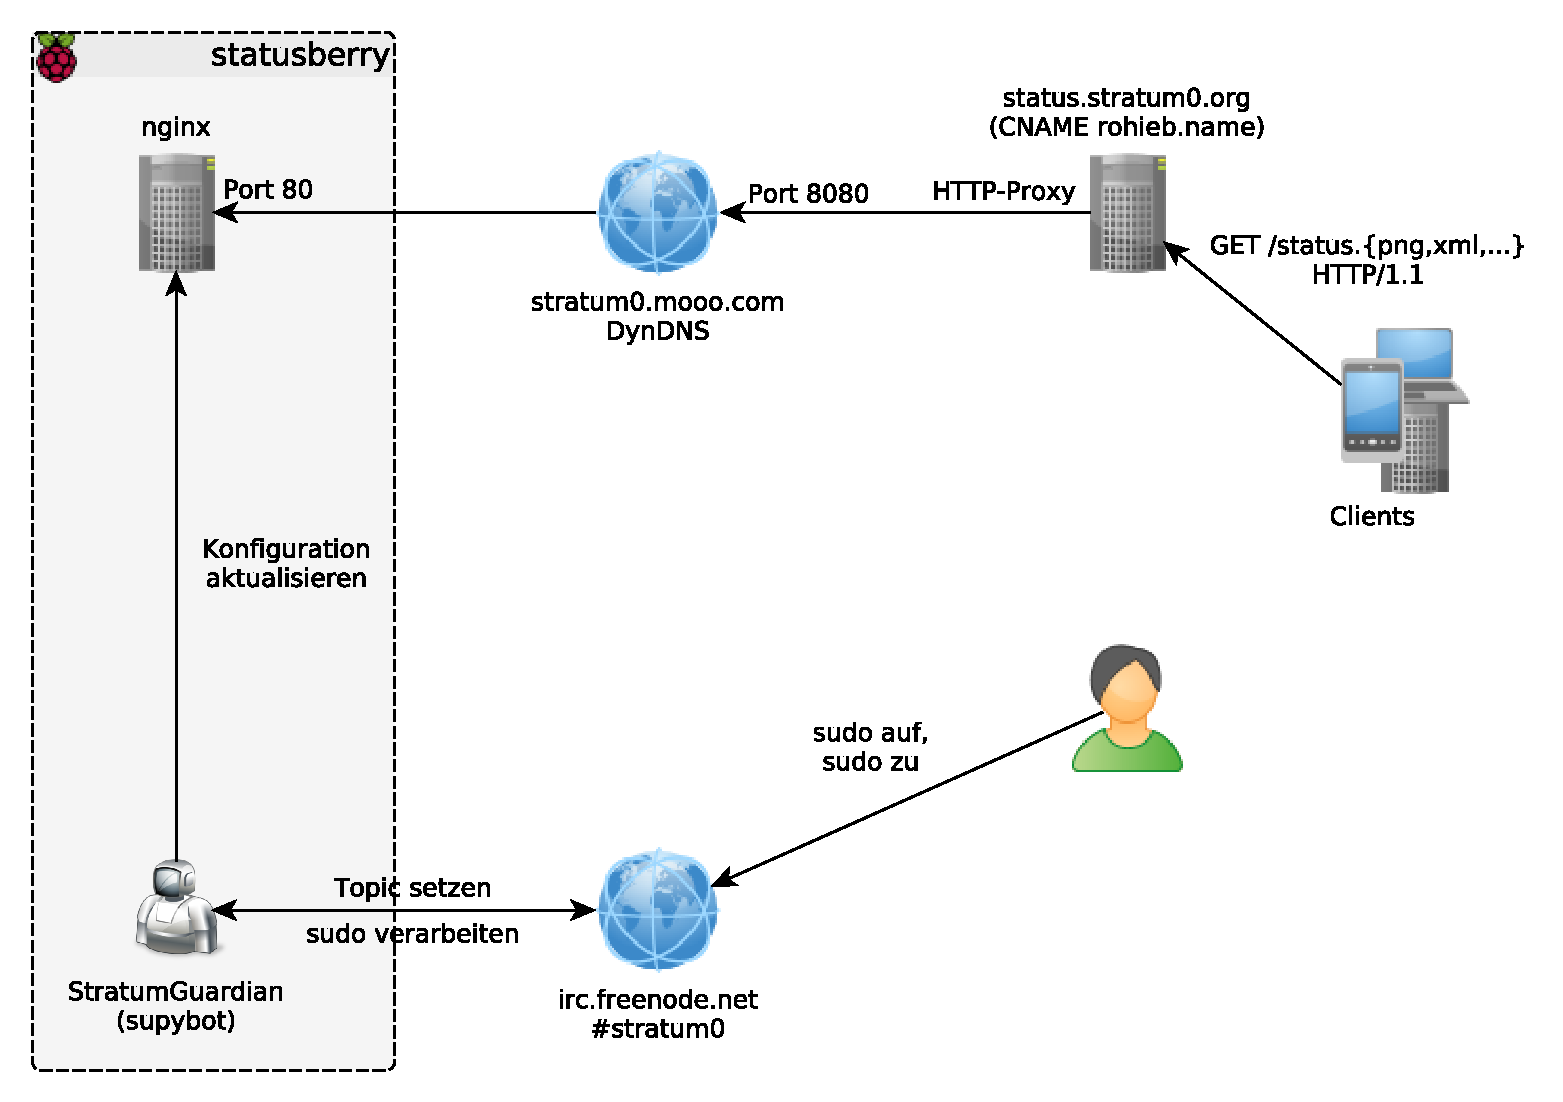
\includegraphics[width=.7\textwidth]{infrastructure-current-phase1.pdf}
  \end{center}

	\begin{itemize}
	  \item Raspberry Pi im Space hostet IRC-Bot und Status per HTTP
		\item \texttt{status.stratum0.org} als HTTP-Proxy für Bequemlichkeit
	  \item aktuell umgesetzt
	\end{itemize}
\end{frame}

\section{Ausblick}
\begin{frame}{Architektur Phase 2: Take back control}
  \begin{center}
    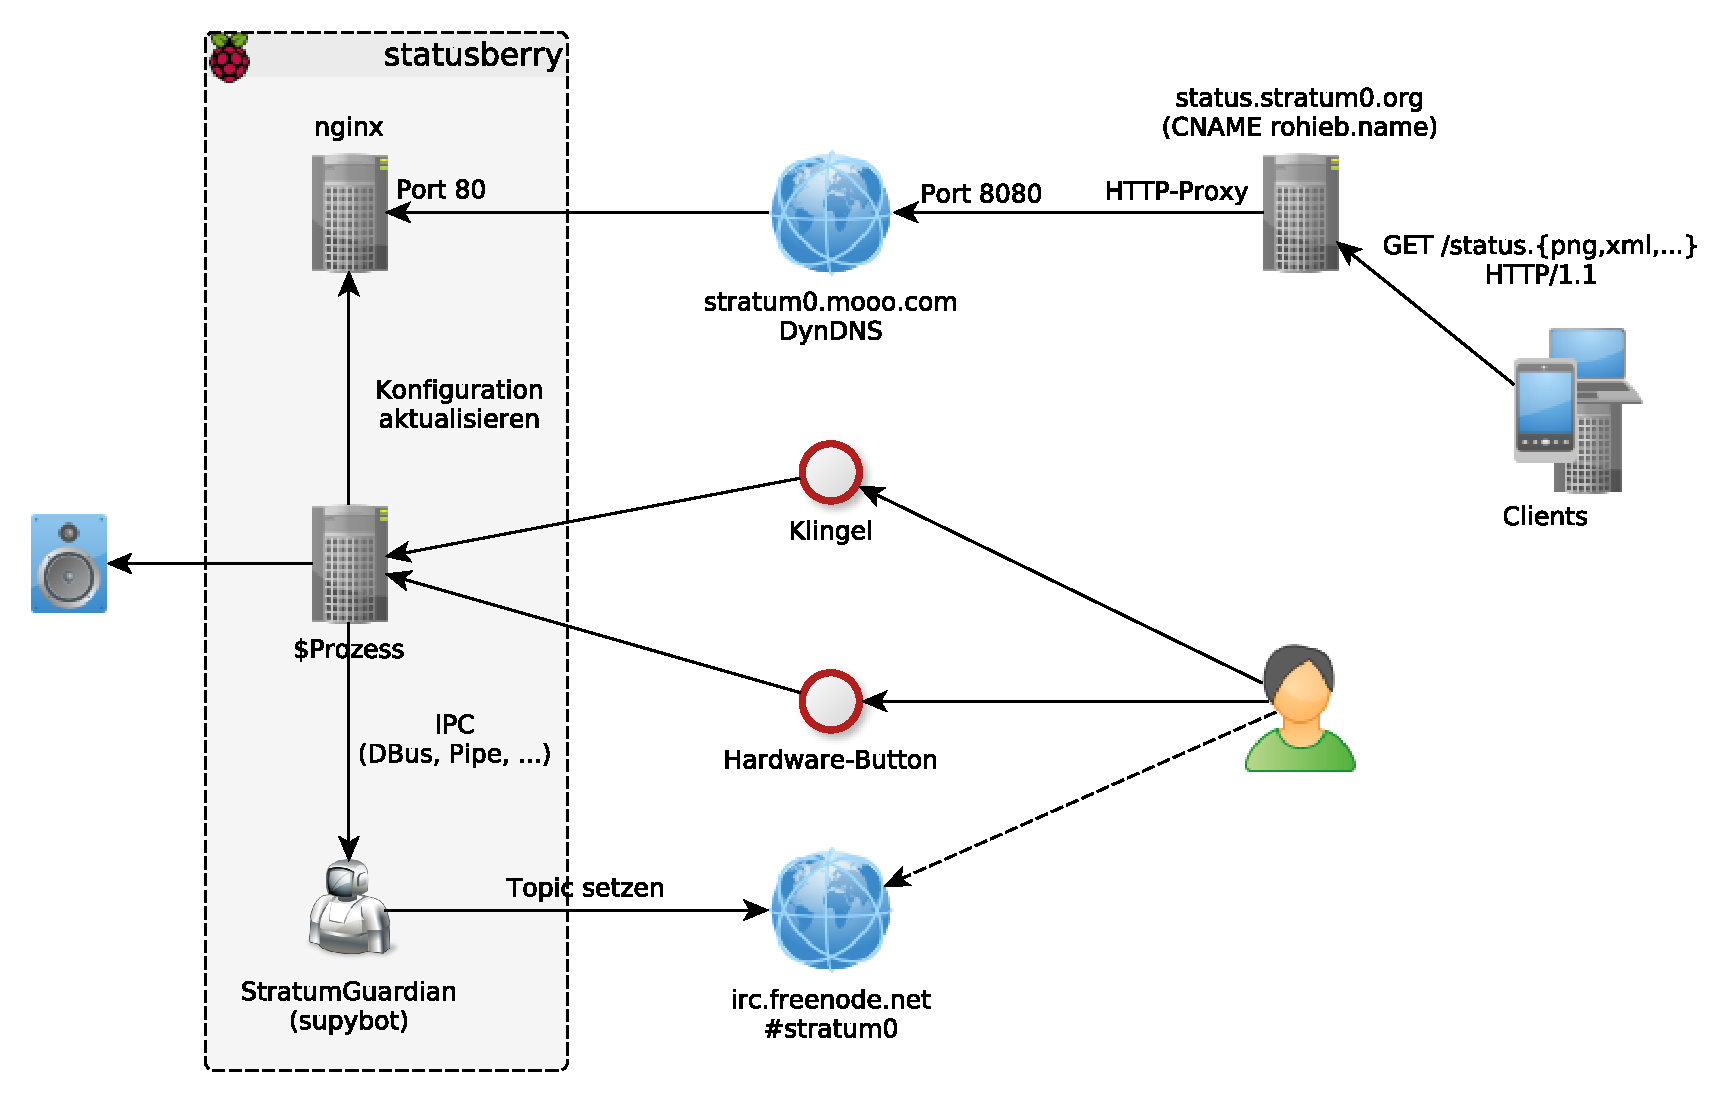
\includegraphics[width=.7\textwidth]{infrastructure-future.pdf}
  \end{center}

	\begin{itemize}
	  \item physischer Taster und Klingel-Events über Raspberry-GPIO
		\item Klingel-Events über Audio (und im IRC?) bekanntgeben
	  \item Integration mit dem Spacekey™-System?
	\end{itemize}
\end{frame}

\section{Software}
\begin{frame}{Software}
  \begin{itemize}
		\item \texttt{statusberry}:
		\begin{itemize}
			\item Debian Squeeze
			\item nginx
			\item supybot mit Plugin \texttt{StratumMonitor}
		\end{itemize}
		\item \texttt{status.stratum0.org}:
		\begin{itemize}
			\item Debian Squeeze
			\item Apache 2 als (SSL-)Proxy
		\end{itemize}
	\end{itemize}
\end{frame}

\section{Bildnachweise}
\begin{frame}
  \centering
  \vfill
  Vielen Dank für die Aufmerksamkeit!
  \vfill
  {\footnotesize Diese Vortragsfolien sind lizenziert unter CC0 (Public Domain)}
  \vfill
	\begin{itemize}
		\item Robot icon: (free for personal use)
			\url{http://www.iconarchive.com/show/real-vista-mail-icons-by-iconshock/robot-icon.html}
		\item Raspberry Pi icon:
			\url{http://en.wikipedia.org/wiki/File:Raspberry_Pi_Logo.svg}
		\item Network icons: yEd,
			\url{http://www.yworks.com/de/products_yed_about.html}
	\end{itemize}
\end{frame}

\end{document}
